\documentclass{article}
\usepackage[utf8]{inputenc}
\usepackage[spanish]{babel}
\usepackage{listings}
\usepackage{graphicx}
\graphicspath{ {images/} }
\usepackage{cite}

\begin{document}

\begin{titlepage}
    \begin{center}
        \vspace*{1cm}
            
        \Huge
        \textbf{Informe Parcial I}
            
        \vspace{0.5cm}
        \LARGE
        Subtítulo
            
        \vspace{1.5cm}
            
        \textbf{Fabian Hoyos}
        
        \vspace{1.5cm}
        
        \textbf{Karen López}
        
        \vspace{1.5cm}
        
        \textbf{Yuribia Arroyave}
            
        \vfill
            
        \vspace{0.8cm}
            
        \Large
        Departamento de Ingeniería Electrónica y Telecomunicaciones\\
        Universidad de Antioquia\\
        Medellín\\
       Abril de 2021
            
    \end{center}
\end{titlepage}

\tableofcontents
\newpage
\section{Sección Introductoria}\label{intro}

El presente trabajo tiene inicio en el parcial 1 de informática 2, de la Universidad de Antioquia, el cual fue propuesto por su respectivo docente Augusto Enrrique Salazar, con el objetivo de evaluar las capacidades, conocimientos, habilidades y destrezas que hemos adquirido los estudiantes durante el curso, tanto en la utilización del lenguaje c++ y Arduino.
Esta evaluación es un gran reto para nosotros como estudiantes, ya que nos servirá para darnos cuenta que tanto hemos aprendido y cuáles son nuestras fortalezas y debilidades realizando el proceso de codificación.
El propósito del examen es lograr realizar un código que muestre un mensaje en una matriz 8x8 utilizando en lenguaje c++, Arduino y el integrado74HC595.


\section{Contenido} \label{contenido}

\subsection{Análisis del Problema}

Se necesita crear una aplicación para un puesto en una empresa llamada Informa 2 S.A.S, donde se requiere desarrollar una animación, la empresa presenta una dificultad y es que tiene un limitante de arduinos, los que poseen no cunetan con suficientes puertos digitales, se debe lograr una animación que muestre letras o una figura que el usuario ingrese. Dicha animación debe tener un patrón de leds. (64leds), se debe conectar y controlarlo con un arduino y el integrado 74HC595, la matriz de leds debe de ser de 8x8, se deben mostrar esos patrones y lograr realizar la conexión del sistema operativo con los 64 leds siguiendo la estructura dada. Para lograr esto se debe realizar una función que pida un patrón por la consola serial y mostrarlo. El objetivo principal es crear una función que muestre cuantos patrones se quieren mostrar y pida los patrones.



\subsection{Esquema para el desarrollo del algoritmo}

Funciones

verificacio:
            Encender todos los leds
imagen:
            Mostrar un patron
publik:
            Publicar secuencia de patrones ingresados por usuario
bindec:
            Convertir binario a decimal
ingfila:    
            Recibe una fila completa del patron y la vuelve decimal
patronU:
            Carga una columna con cada fila como entrada, datos que ingresa el usuario

En la sección de imagen se describe su estructura de manera gráfica.

\subsection{Manual del Usuario}

Los leds estan distribuidos en 8 filas y 8 columnas.
Para ingresar el patrón que se visualizará en el panel de leds, el usuario debe ingresar fila a fila como quiere que esté cada uno de los leds si encendido o apagado.
\vspace{0.5cm}

Se ingresan solo cero(0) para led apagado y uno(1) para led encendido.

\vspace{0.5cm}
Ejemplos:
  \vspace{0.5cm}
Toda la fila apagada: 00000000
Toda la fila encendida: 11111111

El sistema le indicará cuando ingresar cada fila.
En total debe ingresar 8 filas por patron, con combinaciones de ceros y unos.


\subsection{Algoritmo implementado}
// 74HC595 = Pines de Arduino
const int dato = 2;
const int reloj = 3;
const int paso = 4;


//Prototipo de funciones
void verificacion(int); //Encender todos los leds
void imagen(int);//Mostrar un patron
//void publik ();//Publicar secuencia de patrones ingresados por usuario
void bindec(long); //Convertir binario a decimal
void ingfila();//Recibe una fila completa del patron y la vuelve decimal
void patronU(int);//Carga una columna con cada fila como entrada, datos que ingresa el usuario


long result;//variable que guarda el decimal a que corresponde una fila del patron

// Contador de columnas
int j = 0;
int patron[8];

// Contador de duración de secuencia
int k;
int fila[8] = {127, 191, 223, 239, 247, 251, 253, 254};

// columnas de prueba que ayudaron a verificar funcionamiento de leds y codigo
int columnaV[8] = {255, 255, 255, 255, 255, 255, 255, 255}; //encendido completo
int columnaF[8] = {60, 66, 165, 129, 165, 153, 66, 60}; // Emoticon Feliz
int columnaN[8] = {60, 66, 165, 129, 129, 189, 66, 60}; // Emoticon Normal
int columnaT[8] = {60, 66, 165, 129, 153, 165, 66, 60}; // Emoticon Triste

// Se inicializa el 74HC595, y los puertos digitales del arduino
void setup()
{
  Serial.begin(9600);
  Serial.setTimeout(50);
 
  pinMode(dato, OUTPUT); // dato
  pinMode(reloj, OUTPUT); // reloj
  pinMode(paso, OUTPUT); // paso
  
  pinMode(13, OUTPUT);
 }

void loop()
{    
   //Serial.println(binario);

    imagen(patron);
  //verificacion(columnaV); //Encendido total con la función verificación
  //verificacion(columnaV);//Encendido total con funcion imagen
   //verificacion(columnaN); //emoticon cara normal
  // verificacion(columnaT); //emoticon cara triste
  //verificacion(columnaF); //emoticon cara feliz
  }
  
// Funcion para imprimir un patron, definido por el vector columna(N,T,F y lo que ingrese el usuario)
//Se usa el nombre del vector de columnas, como puntero de la entrada cero del mismo vector
void patronU(int patron[8]){
  for(int f=0;f<8;f++)
  {
    Serial.print("Ingrese fila "); Serial.print(f+1);Serial.println(" del patron: ");
  	ingfila();
    patron[f]=result;
    //Serial.print(patron[f]);
  }
}

void imagen(int tipo[8])
{
  patronU(patron);
  for(k = 0; k<100; k++)
  {
    for(int i=0; i<8; i++)
    {
      digitalWrite(reloj, LOW);//Se baja con un pulso el reloj
      shiftOut(dato, paso, MSBFIRST, *(tipo+j));//Trae lo que hay en el vector columnas, por medio del contenido de su puntero
      shiftOut(dato, paso, MSBFIRST, fila[i]);//La fila trae tiempos de duración de la secuencia
      digitalWrite(reloj, HIGH);
      j++;
    delay(0.1);  
    }
    j = 0;
  }
 }

//Se usa el nombre del vector de columnas, como puntero de la entrada cero del mismo vector
void verificacion(int patron[8])
{
 for(int k = 0; k<100; k++)
  {
    for(int i=0; i<8; i++)
    {
      digitalWrite(reloj, LOW);//Se baja con un pulso el reloj
      shiftOut(dato, paso, MSBFIRST, *(patron+j));//Trae lo que hay en el vector columnas, por medio del contenido de su puntero
      shiftOut(dato, paso, MSBFIRST, fila[i]);//La fila trae tiempos de duración de la secuencia
      digitalWrite(reloj, HIGH);
      j++;
    delay(0.1);  
    }
    j = 0;
 }
  
}
//conversor de binario a decimal
void bindec(long numero){
    long resto=0, x=1;
    int digito[8];
  
    //cout <<"Ingrese binario: ";
    //cin>> binario;
    for(int i=0;i<8;i++){
        digito[i] =numero%10;
        numero /=10;
    }
    for (int i=7; i >=0; i--){
        result = (resto *2)+digito[i];
        resto = result;
     }
       // Serial.println(result); //imprime decimal de entrada para pruebas
 }            

/*//Funcion para mostrar una secuencia de patrones
void publik (){ }// En desarrollo
/*Esquema en C++
void dinamica(){
    int **punteroP; //Puntero que apunta a puntero de filas en matriz "patrones"
    int nF, nC = 8; //número de Filas de la matriz "patrones", las columnas son 8.
    cout<<"Ingrese la cantidad de patrones que quiere mostrar: ";
    cin>>nF;
    //Reservar memoria dinamica para la matriz de patrones
    punteroP = new int*[nF]; //para las filas
    for(int i=0;i<=nF;i++){
        punteroP[i] = new int[nC];//Para las Columnas
      }
    //Solicitar elementos para llenar la matriz
    for (int i=0; i<nF;i++){
        imagen();
        for (int j=0;j<nC;j++){
            *(*(punteroP+i)+j)= patron[j];//puntero matriz[i][j]

        }
    }
}*/
//Funcion que llena una fila del patron
void ingfila()
{
	long nBin=10000000, binario = 0;
  	//Serial.println("Ingrese la fila: ");
 	while(Serial.available()==0){};//Espera que se ingrese dato
 	if (Serial.available())
   	{
      char datos[8];
      size_t count = Serial.readBytesUntil('\n', datos, 8);
      for (int i = 0; i< count; i++) 
      {
        //Serial.print(datos[i]);
        //Serial.println();
        if(int(datos[i])==49)
        {
          binario = binario + nBin;
        }
         nBin = nBin/10;  
	}
   Serial.println(binario);//Imprime binario y va mostrando patron ingresado por usuario en monitor
   bindec(binario);   
   }
  delay(0.1);
  
} 

\subsection{Problemas que se presentaron}

Los problemas que más afectaron este proyecto fueron el poco conocimiento en electronica, lo que nos llevo a cambiar en varias ocaciones el modelado del prototipo.
 
 \vspace{1.5cm}
 
 Otro problema fue el poder hallar una manera eficiente de que el usuario ingresara los datos del patrón, debido a que el arduino recibe la información caraacter a caracter y tipo ascii, así que si el usuario ingresa algo en pantalla hay que modelar esa información para tener el resultado esperado, y se tuvo que estudiar bastante ese tema.
 
  \vspace{1.5cm}
 Y el hecho de que la plataforma tinkercad no ha estado muy estable, y tocaba cargar frecuentemente la página web para seguir trabajando, retraso bastante las tareas.


\subsection{Evolución y consideraciones}

\section{Inclusión de imágenes} \label{imagenes}

En la Figura (\ref{fig:estructura}),es el prototipo que se empezó a diseñar.

\begin{figure}[h]
\includegraphics[width=4cm]{estructura.jpg}
\centering
\caption{Logo de C++}
\label{fig:estructura}
\end{figure}

En la Figura (\ref{fig:prueba_corriente1}),es el prototipo que se empezó a diseñar.

\begin{figure}[h]
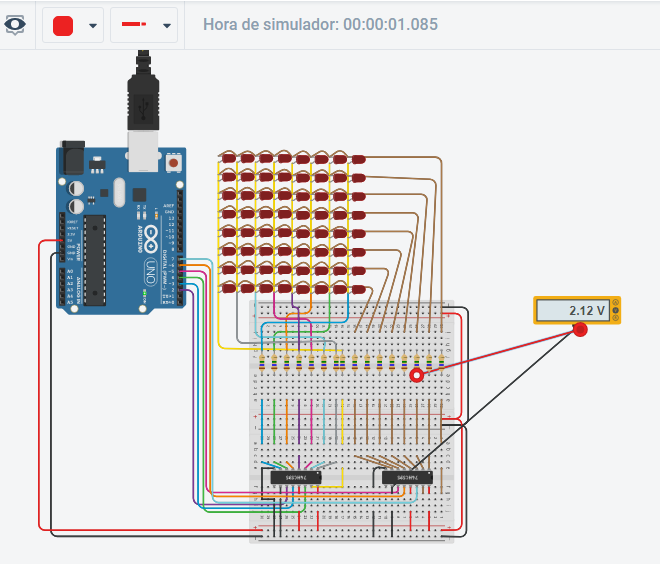
\includegraphics[width=4cm]{prueba_corriente1.png}
\centering
\caption{Logo de C++}
\label{fig:prueba_corriente1}
\end{figure}

En la Figura (\ref{fig:primer_patron}), se presenta el prototipo final.

\begin{figure}[h]
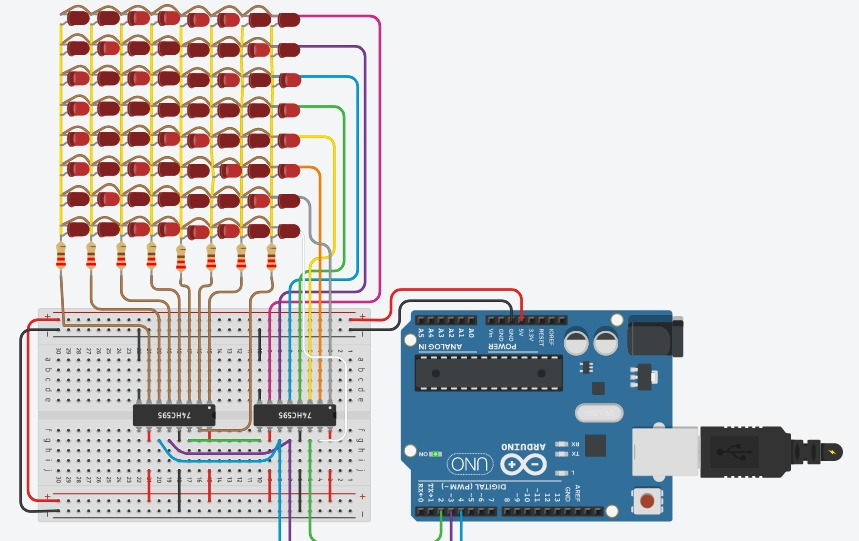
\includegraphics[width=4cm]{primer_patron.png}
\centering
\caption{Logo de C++}
\label{fig:primer_patron}
\end{figure}

Las secciones (\ref{intro}), (\ref{contenido}) y (\ref{imagenes}) dependen del estilo del documento.

\bibliographystyle{IEEEtran}
\bibliography{references}

\end{document}
